% !TeX root = /../Report.tex

\chapter{Introduction}\label{sec:introduction}
This template is meant to be used for semester, bachelor, and master theses written at the Sensory-Motor Systems Lab (SMS), ETH Zurich. The template includes several examples of equations, figures, tables, etc. in order to act as a {\it very} short introduction to \TeX\! and \LaTeX. Yet, the template is also provided to ensure that all written work in \LaTeX ~at SMS shares identical formatting.
This template is based on the IMRT\footnote{Institute for Dynamic Systems and Control, ETH Zurich; www.imrt.ethz.ch} \LaTeX ~template by Eric Mueller (2009) and Soren Ebbesen (2013).

\section{The Preamble}\label{sec:preamble}
The preamble of the \LaTeX\! template defines the font size, page layout, language, report type, title, and author(s) of the report. The preamble of the current template is shown below. It should be more or less clear how you need to modify the preamble to fit your needs; if not, consult your supervisor.
%\lstset{language=TeX,numbers=none}
%\begin{lstlisting}[frame=lines]
\begin{verbatim}
\documentclass[10pt,twoside,a4paper,fleqn]{report}

\usepackage[english,st,balgrist]{ethsms} % Special SMS styles and commands      	
								 % {german}/english: language of headings, etc.
								 % {st}/bt/mt: {semester}/bachelor/master thesis
								 % {balgrist}/nobalgrist: {include Balgrist Logos}/exclude Balgrist Logos
							

% Title page (please fill in)___________________________________________________
\title{SMS \LaTeX\ Thesis Template v.1.0}


\studentA{Hans Muster}
\ethidA{97-906-739}
\semesterA{5}
\emailA{muster@student.ethz.ch}

%\studentB{Second Student}
%\ethidB{12-345-678}
%\semesterB{9}
%\emailB{second@student.ethz.ch}

\supervision{First Supervisor\\ Second Supervisor}
\date{March 2011}
 \end{verbatim}
%\end{lstlisting}

The style \texttt{ethsms.sty} enforces certain changes to the original \texttt{report} class, e.g., the title page. The style accepts three options. The first option lets you choose the language of your report, i.e., the language of the title page, headings, info-page, etc. Valid options are: \texttt{german} (default) and \texttt{english}. The second option defines the type of report which will be printed on the title and info page. Valid options are: \texttt{st} (default), \texttt{bt}, and \texttt{mt} for semester, bachelor and master thesis, respectively. The third option is to decide which logo configuration you will have on your title page.
Valid options are:  \texttt{balgrist} (default) and  \texttt{nobalgrist}, with this option you can choose to either include the UZH and Balgrist logos or not.
For instance, if you will be writing a master thesis in English and wish to add the UZH and Balgrist Logos, use
\begin{verbatim}
 \usepackage[english,mt,balgrist]{ethsms}
\end{verbatim}



\section{Compiling With pdfLatex}\label{sec:pdfLatex}

Some packages (pstricks) used for this template do need to be compiled to from latex to dvi to pdf.
If you want to use ''pdfLatex'' (as I do), then you need an additional setting to allow your compiler (for me it is Miktex on Windows) to create some ``in-between'' files and access them afterwards.

For TexWorks the required additional setting is shown in figure~\ref{img:pdfTexWorks}.
If you use the combination of ''pdfLatex+MakeIndex+BibTex'' the setting is slightly different, see figure~\ref{img:pdfTexWorks2}.

For other platforms and/or editors you can find information here: 

\url{http://tug.org/PSTricks/main.cgi?file=pdf/pdfoutput#texworks}

\begin{figure}[ht]
   \centering
   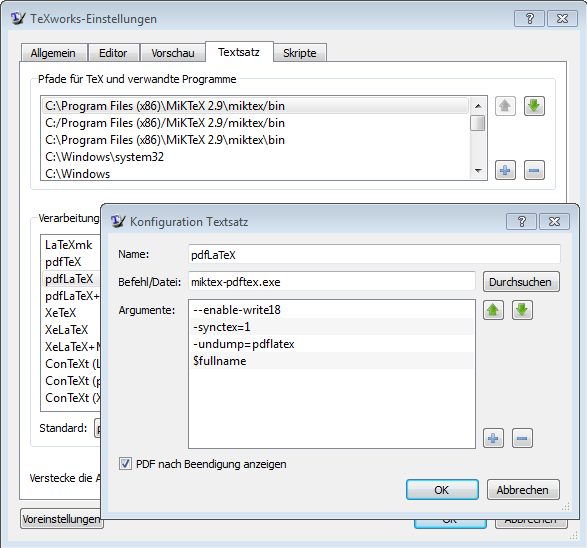
\includegraphics[width=0.9\textwidth]{img/pdfLatexSettingsForTexWorks.PNG}
   \caption{pdfLatex Settings in TexWorks}
   \label{img:pdfTexWorks}
\end{figure}

\begin{figure}[ht]
   \centering
   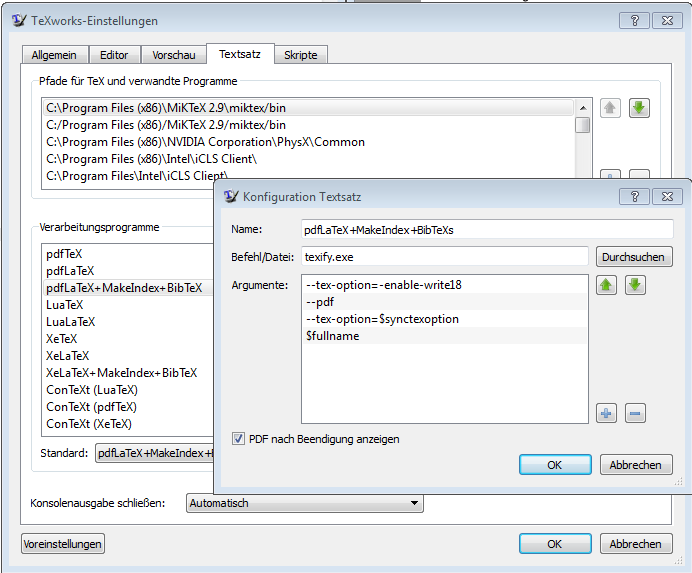
\includegraphics[width=0.9\textwidth]{img/pdfLatexMakeIndexBibTexSettingsForTexWorks.PNG}
   \caption{pdfLatex+MakeIndex+BibTex Settings in TexWorks}
   \label{img:pdfTexWorks2}
\end{figure}